\subsection{Analiza korelacji tweetów pomiędzy analizowanymi kontami }
Posiadając zbiór postów analizowanych kont, który zawiera nie tylko posty oryginalnie stworzone przez te konta, ale również retweety postów z\,innych kont, chciano sprawdzić, czy istnieją relacje pomiędzy badanymi kontami. 
\par
Dokonując tej analizy chciano zbadać dwie rzeczy. Pierwszym celem było zbadanie, czy badane konta udostępniają nawzajem swoje tweety, oraz jeśli tak to czy należą one do tej samej klasy czy do różnych klas. Drugim celem było sprawdzenie czy istnieją konta, nie będące uwzględnionymi w\,obecnym zbiorze klasyfikacji, z\,których konta, które znajdują się w\,tym zbiorze udostępniają treści. Dzięki temu planowano wykryć niebezpośrednie relacje pomiędzy badanymi kontami.
\par
Aby ułatwić tę analizę stworzono wizualną reprezentację sieci udostępnień tweetów przez konta (Rysunek \ref{fig:connectedaccounts}). Zawarto w\,niej wszystkie konta ze zbioru klasyfikacji, które udostępniły przynajmniej jeden post opublikowany oryginalnie przez inne konto ze zbioru. Na tym samym rysunku przedstawiono również inne konta, które były udostępnione przynajmniej 30 razy przez któreś z\,badanych kont. 
\par
Na rysunku konta zostały przedstawione jako wierzchołki, zakodowane kolorem w\,zależności od klasy, do której należą. Konta nie należące do żadnej z\,klas zostały opatrzone etykietą ‘Inne’. Należą one do grafu skierowanego, gdzie łuk istnieje między wierzchołkiem A\,a wierzchołkiem B, gdy konto A\,udostępniło post konta B. Na rysunku grubość łuków wyraża jego wagę liczoną jako liczbę udostępnionych postów. Jest to jednak wartość tyko poglądowa, ponieważ skala możliwych wartości była zbyt duża, aby czytelnie odzwierciedlić ją na rysunku. 
\begin{figure}[!h]
	\centering 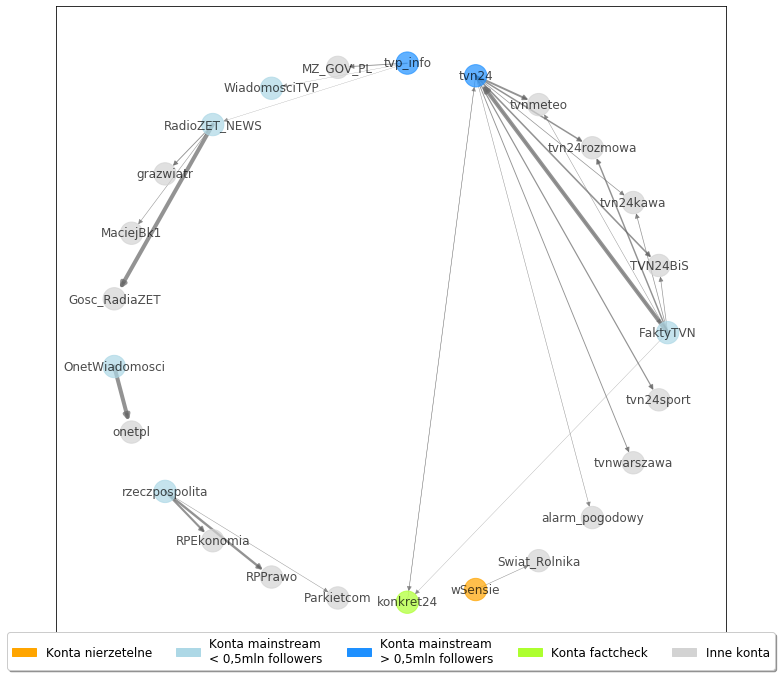
\includegraphics[width=1.0\linewidth]{img/results/connectionbetweenaccounts.png}
	\caption{Sieć udostępnień tweetów przez konta z\,podziałem na  klasy} \label{fig:connectedaccounts}
\end{figure}
\par
Dzięki stworzonemu rysunkowi, przedstawiającemu sieć udostępnień tweetów pomiędzy znaczącymi kontami można zauważyć, że generalnie nie ma zbyt wiele relacji pomiędzy analizowanymi kontami. Na 28 kont, w\,prezentowanej sieci znalazło się tylko 10 z\,nich. Co można zauważyć, to fakt, że najczęściej udostępniane są treści należące do tej samej grupy wydawniczej. Najlepszym przykładem tutaj jest grupa TVN, gdzie na koncie tvn24 oraz FaktyTVN udostępniane są posty z\,siostrzanych serwisów należących do tej samej grupy. To samo zjawisko występuje również dla pozostałych kont. 